\documentclass[12pt,letter]{article}

\usepackage{amsmath}
\usepackage{natbib}
\usepackage{graphicx}
\usepackage{booktabs}
\newcommand{\tabitem}{~~\llap{\textbullet}~~}

\title{Hierarchical benchmarking for lava flow simulations}
%\date{}
%\author{Jacob Richardson, Laura Connor\\ Charles Connor, Sylvain Charbonnier}
\author{Jacob Richardson}

\usepackage[margin=1.5in]{geometry}
\usepackage{setspace}
%\doublespacing

%\usepackage{lineno}
%\linenumbers

%Geology Papers are limited to ~5000 words

\begin{document}

\maketitle

\section*{Abstract}
	Modeling lava flows through cellular automata (CA) methods enables a computationally inexpensive means to quickly forecast lava flow paths and ultimate areal extents. A CA program has been created in the program language C that is modular, which enables a combination of governing CA rules to be evaluated against each other. My objective is to find a successful combination of automata behaviors that accurately forecasts lava inundation and behaves like a bingham fluid. To fulfill this objective, four benchmarking levels have been devised to test lava spreading algorithms against increasingly complex tests. These levels are 1) verification of the code by testing for conservation of mass; 2) testing for flow self-similarity given inconsequential variations of arbitrary surfaces; 3) testing for replication of Bingham flow morphology on simple surfaces and; 4) testing for replication of real lava flow morphologies on pre-eruptive surface models. Currently the best-fitting lava spreading algorithm for these four benchmarking tests might be an algorithm which spreads lava proportional to slope and where each automaton is able to spread lava in 8 directions.

\section{Introduction}
	Lava flows as a gravity current on the surface of the Earth when liquid magma is effused at the surface with little or no explosivity. In the vacinity of active volcanoes, lava flows represent significant long term impact to infrastructure. In the past, lava flow hazard has been mitigated with the construction of physical diversions and at least once in 252 AD by the supernatural grace of St. Agatha of Sicily who died the year prior. Modern science suggests, however, that forecasting the flow path of lava from active volcanoes might be more useful than St. Agatha for communities impacted by effusive volcanism.

	Methods of forecasting lava flows range from simple predictions using empirical relationships between magma flux and flow length \citep{Glaze2003}, to 1-D numerical solutions such as FLOWGO \citep{harris2001flowgo}, to advanced computational fluid dynamics codes like lavaSIM \citep{hidaka2005vtfs}. All modern numerical flow models by nature trade precision in simulating physical processes with computer run-time, so that while FLOWGO is relatively fast it only predicts downslope flow length, while lavaSIM solves Navier-Stokes equations to produce a 3-D flow distribution at the expense of large computational requirements.
	
	Cellular Automata (CA) methods have been developed to simulate fluid flow, including lava spreading \citep{barca1994cellular}. In contrast to CFD codes, these do not generally attempt to compute Navier-Stokes equations but instead abstract many physical parameters, such as viscosity and temperature, into more or less empirical rules. The benefit of CA methods for simulating lava flows is most noticeable in the reduced computer time necessary for simulation compared to CFD methods.

	CA in lava flows has historically been defined as a 2-dimensional space, which is divided into equal-area cells, such as those found in a common digital elevation model (DEM). Within the location of each cell is defined an ``elementary automaton'' (\textit{ea}) that has a set of properties, is governed by a set of global rules, and has a set list of neighboring automata. While the behavior rules each \textit{ea} is identical to those of all other automata, its behavior is only dictated by local phenomena. Specifically, the amount of lava that flows in or out of an \textit{ea} will depend on properties such as lava thickness and elevation within it and its neighbors. Traditionally, CA is specified as a series of states:
	\begin{equation}
		\mathbf{A} = \mathrm{\{E,S,X\}}
	\end{equation}
	where E is the set of point locations of cellular automata in \textbf{A}, S is the set of substates within each automaton, and X is a set of automata within the neighborhood that influence the state of each automaton \citep{barca1994cellular}. Specifically, for a cell, E is a coordinate pair (i,j) denoting the row and column address of that cell in the larger grid. The set S fundamentally includes S$_e$, the underlying elevation of an automaton; S$_h$, the thickness of lava within the cell; and S$_h0$, the critical thickness, above which lava will spread from a cell. Some algorithms include S$_T$, or the cell temperature in this set. X, in a four-connected CA system is given as \{(0,1), (0,-1), (1,0), (-1,0)\}, where (0,0) is the location of an automaton under evaluation. The implementation of these sets within the CA structure \textbf{A} is described in detail in Section \ref{sec:MOLASSES}.
	
	Multiple CA lava flow algorithms exist, such as SCIARA \citep{crisci2004simulation}, MAGFLOW \citep{del2008simulations}, ELFM \citep{damiani2006lava}, and LavaPL \citep{connor2012}. These algorithms are variations on a theme, where the largest difference between each is how lava is distributed from one automaton to its neighbors. For instance, three versions of SCIARA allow for lava to spread in cardinal directions \citep{barca1994cellular}, in hexagonal directions \citep{crisci2008lava}, or in directions based on an inherent velocity calculated in an eulerian way for each automaton \citep{avolio2006sciara}. MAGFLOW and ELFM by contrast to the original SCIARA algorithm implements 8 directions of spreading. LavaPL and SCIARA both spread in four directions but the apportionment of lava from one automaton to neighbors is based on a different algorithm.

	While several lava flow simulators now exist, each have been made and tested with different lava flows or aspects of flows in mind. Because of this, selecting a specific algorithm to effectively model lava flow hazards can be a necessary, if unwanted challenge. To address this problem, we propose a hierarchical benchmarking scheme to objectively rank different flow spreading algorithms. This hierarchy tests simulated output against increasingly complex tests, from simply conserving mass to replicating the paths and ultimate areal extents of real lava flows. These benchmarking methods can be applied to any flow algorithm that provides at least a list or map of inundated locations over various topographies.

	Multiple lava flow algorithms are tested using a new modular lava flow code, which I have named MOLASSES (tentatively standing for \textit{MOdular LAva Simulation Software in Earth Science}). This code, implemented in C, is a Cellular Automata code which tracks a population of equal-area spaced cells over a grid, that is defined by a digital elevation model (DEM). These cells may or may not be inundated with lava and they are governed by universal rules which dictate if and how lava can move into and out of them, in line with the CA method described above. Because MOLASSES has been designed in a modular way, it is relatively quick to assign spreading rules and modify the flow algorithm. Using this code while changing methods of lava distribution enables code output in a constant format, which simplifies the comparison of methods.


	\section{A Benchmarking Hierarchy}
	
	The strategy implemented in this paper follows the advice of \citet{bayarri2007framework} for validating computer models, namely ``1) defining the problem; 2) establishing evaluation criteria; 3) designing experiments; 4) approximating computer model output; 5) analyzing the combination of field and computer run data.'' The sixth step in their validation process, feeding results back to revise models, has been done informally in determining how to alter spreading algorithms in future benchmarking attempts. Each level below presents a problem for a lava spreading algorithm to complete. These fundamental problems (e.g. replicating a Bingham flow) are evaluated using simple tests that demonstrate the problem. The relevant model output for each of these tests is a list of locations that have been inundated by lava. Planned future tests will also require the thickness of lava at each location inundated by lava in a given test. Lastly, tests compare model output with expected output. After verification (Level 0), the first validation level tests model results with other model results; the second tests model output against expected analytical solutions; and the third level tests model output from field data.

	\subsection{Level 0: Conservation of Mass}
		\subsubsection{Conservation of Mass}\label{test:CoM}
			Before the results of a lava flow simulation can be benchmarked or validated, it must be verified to at least prove that conservation of mass is preserved. A lava flow simulation will therefore not be tested against the following benchmark tests until this conservation of mass requirement is shown to be fulfilled. By the design of MOLASSES, this test is performed for each simulation by summing the total volume delivered to vents, as specified by the user in a configuration file, and comparing it to the sum of volume in all cells at the end of the simulation. If the quantities are not equal, the test fails, mass is not conserved, and the code is not able to be validated.
	
			\begin{center}
				\begin{tabular}{l}
					\toprule
					\textbf{Test \ref{test:CoM} Algorithm}\\
					\midrule
					Implemented in MOLASSES:\\
					1.~$V_{in}\leftarrow \displaystyle\sum^{Vents} V_{v}$, for each vent, $v$.\\
					2.~$V_{out}\leftarrow \displaystyle\sum^N V_{c}$, for each cell, $c$.\\
					3.~Test $V_{in}-V_{out}=0$\\
					~\tabitem \textit{True}: Success\\
					~\tabitem \textit{False}: Failure\\
					\bottomrule
				\end{tabular}
			\end{center}

	\subsection{Level 1: Self similarity given ersatz parameter space variation}
		The first level of model validation tests that a lava spreading algorithm remains the same given dummy, or ersatz, changes in parameter space. To evaluate the performance of algorithms at this level, parameters such as elevation values of the underlying surface model are changed in a way that should not effect model output. Model output is then compared with model output from effectively identical parameters to see if model output is also effectively identical. For instance, a slope to the west and an identically dipping slope to the east should produce lava flows of equal length and shape, all other flow parameters remaining equal. Because the larger goal of this level is simply to test the ability for algorithms to remain unchanged and they are not yet expected to be realistic flows, parameter space can be arbitrarily assigned initially.
		
		\subsubsection{Rotating Sloped DEM}
			Miyamoto and Sasaki (1997) performed a simple validation test on two CA-like flow simulators (Ishihara, 1990 and Miyamoto and Sasaki, 1997) where a sloped DEM was rotated 45 degrees from ``south'' to ``southeast''. This test was performed to verify that the flow models had the same run-out regardless of the arbitrary slope direction. The DEM rotation scheme by Miyamoto and Sasaki (1997) is adopted and expanded, so that a DEM with a simple sloping face is rotated 180 times at an increment of 2$^{\circ}$. The farthest point of a simulated flow from a given model is reported for each slope direction. A perfect flow model will have no variation in distance traveled with respect to slope direction.

			\begin{center}
				\begin{tabular}{l}
					\toprule
					\textbf{Rotating Slope Test Algorithm}\\
					\midrule
					1.~Assing constant DEM and Flow parameters\\
						~\tabitem $\phi:=$DEM slope\\
					2.~Write configuration file\\
					3.~For 180 azimuths, $\theta$, from 0-360$^{\circ}$\\
						~\tabitem create DEM dipping $\phi$, $\theta$ from N.\\
						~\tabitem run \textbf{MOLASSES} over DEM\\
						~\tabitem $l$:=i,max dist$\{C_0-C_i\}$\\
						~\tabitem $d_{l,\theta}$:=dist$\{C_0-C_l\}$\\
						~\tabitem $w$:=i,max dist$\{\overrightarrow{C_0C_l}-C_i\}$\\
						~\tabitem $d_{w,\theta}$:=dist$\{\overrightarrow{C_0C_l}-C_w\}$\\
					4.~Find average, $\mu$, standard deviation, $\sigma$ of $d_l$,$d_w$\\
						~\tabitem CV$_l$:= $\sigma_l/\mu_l$\\
						~\tabitem CV$_w$:= $\sigma_w/\mu_w$\\
					5.~Define success, failure based on CV.\\
					\bottomrule
				\end{tabular}
			\end{center}


		\subsubsection{Potential Level 1 Tests}
		\paragraph{Scaling Spatial Resolution}
			A second DEM-altering test would be where lava flows will be simulated over surfaces of different spatial resolutions. These surfaces could either be flat or a slope. The largest inhibitor of this test currently is a parameter in MOLASSES known as the Pulse Volume. At differing spatial resolutions, the choice of Pulse Volume changes the flow runout length in a way that is not necessarily proportional to resolution, so it is not yet known how to choose this parameter for this test.

	\subsection{Level 2: Replication of flow morphologies on simple physical surfaces}
	
	The second benchmarking level is the first step in validating lava flow algorithms against realistic flow expectations. Instead of parameter space being arbitrarily defined, which was the case in Level 1, the defined parameter space informs tests at this level as to what the model output should be.
	
		\subsubsection{Flow areal extent approximates a circle on a flat plane}\label{test:Bing_circ}
		
			As lava flows on a large scale are well described as Bingham fluids, a flow simulation can be further tested by being compared to analytical solutions or experimental observations of these fluids under simple conditions. For instance, a lava flow on a perfectly flat surface might be expected to create a circular areal extent. Another example is that lava flows are expected to thicken up-slope when encountering a vertical obstacle.
	
			Here we measure flow algorithm performance on a flat surface from a single vent source location. Two tests measure this performance. First, it is expected that the flow will be circular. To measure the extent to which the simulated flow replicates a circle, we measure the inundated area and compare that to the area of a circle which circumscribes the flow exactly. This can be described as
			\begin{equation}
				Fit = \frac{A_{flow}}{\pi d_{max}^2}
			\end{equation}
			where $d_{max}$ is the farthest extent of the simulated flow from the vent. A perfect match to a circle would result in a $Fit=1$. With the same maximum distance from the vent (i.e. the distance from the center to a vertex) a perfect square would cover 64\% of the area of a circle, ergo $Fit=0.64$. An octagon would have a fit of 0.90. We consider a model to successfully pass this test if it produces a flow of $Fit>0.90$, or if the flow approximates a circle better than an octagon. The model fails this test if if produces a flow of $Fit<0.64$, where a square better describes a circle than a flow generated from the model.

			\begin{center}
				\begin{tabular}{l}
					\toprule
					\textbf{Test \ref{test:Bing_circ} Algorithm}\\
					\midrule
					1.~Create flat DEM with spatial resolution, $R$\\
					2.~Write configuration file for flow\\
					3.~Run \textbf{MOLASSES} over DEM\\
					4.~Define results:\\
						~\tabitem $d_{max}$~:=~max dist$\{\overrightarrow{C_0C_l}-C_i\}$\\
						~\tabitem $N$~:=~Number of cells, $C$, inundated\\
					5.~Compare $N$ with $N_{circle}$,$N_{octagon}$,$N_{square}$ where:\\
						~\tabitem $N_{circle}:=\pi d_{max}^2/R$\\
						~\tabitem $N_{octagon}:=2.82842 d_{max}^2/R$\\
						~\tabitem $N_{square}:=2d_{max}^2/R$\\
						~1. If $N>N_{octagon}$: Success\\
						~1. If $N<N_{square}$: Failure\\
					\bottomrule
				\end{tabular}
			\end{center}


		\subsubsection{Potential Level 2 Tests}
			\paragraph{Flow thickness profile approximates a Bingham fluid on a flat plane}
				A second flat-surface test compares the averaged flow thickness profile away from the vent from a theoretical axisymmetric thickness profile of a viscoplastic fluid. The analytical solution for height with respect to radius is given by Griffiths (2000) as
				\begin{equation}
					h(r)^2 = \frac{2\sigma_0(R-r)}{\rho g}
				\end{equation}
				where $\sigma_0$ is the yield strength of the flow, R is the outer radius, and $\rho$ is the fluid density. As $\sigma_0$ and $\rho$ are not generally given \textit{a priori} in CA codes, we will use $C$ where $C=\sigma_0/\rho$ as a placeholder. For each model, a flow will be generated on a flat plane, a $\chi^2$ test will be used to find the best fit $C$, which will have the least error between the analytical and the simulated axisymmetric thickness profiles, and the misfit will be reported.

			\paragraph{Flow morphology approximates a Bingham fluid on a slope}
				Another Level 2 test tests algorithms' abilities to recreate viscoplastic flow morphology for a flow on a slope. Following Osmond and Griffiths (2001), the areal footprint of a yield strength fluid can be solved by comparing its strength, total volume, and the underlying surface slope. Because it might be hard to scale the model to findings from Osmond and Griffiths \textit{a priori}, the best fitting Bingham parameters can be found for a given model output and the error from this best fit can be compared to the error from the output of other flow algorithms. This would likely also inform how flow spreading algorithms scale to real world dimensions.

			\paragraph{Thickness profile approximates a Bingham fluid behind an obstacle}
				Bingham fluids flowing over a significant obstacle on a slope exhibit a bow shock upslope from the obstacle. Using an obstacle such as a cylinder or a triangle, the thickness profile along the flow axis upslope of the obstacle as determined by a numerical solution can be compared with model output from a flow algorithm.



	\subsection{Level 3: Replication of real lava flows over complex topography}
		The recent availability of global or near-global topographic datasets, such as SRTM or ASTER GDEM has enabled the direct observation of the underlying surface of even more recent lava flows. The extents of lava flows such as the 2012-3 Tolbachik lava flow, in conjunction with available pre-eruption DEMs, is the final benchmarking test for lava flow algorithms. At this level, model inputs must reflect reality, which naturally makes parameter spaces used in applicable tests more complex than those used in previous levels. Ultimately, if a lava spreading algorithm succeeds at this level after performing well in previous levels, the algorithm is considered validated against field data.

		\subsubsection{2012-3 Tolbachik, Russia lava flows}\label{test:Real_Tolbachik}
			The goodness of fit between a simulated flow and a mapped lava flow can be simply measured by the Jaccard coefficient. This parameter is the ratio of the intersection area inundated by both the simulation and the real flows by the union area inundated by either. To illustrate, this test has been performed recently by Kubanek et al. (submitted) for the 2012-3 Tolbachik flow where a MOLASSES model configuration, explained later, produced a lava flow with a 59\% fit to the mapped flow. This result means that 59\% of the area inundated by either the simulated flow or the mapped flow, the union, was inundated by both the simulated and the mapped flows. Conversely, 41\% of the area was either modeled to have been inundated but wasn't or was modeled to be lava-free but actually was inundated by lava. These are generally known as false positives or false negatives, respectively.
			

			%Go on about how the Jaccard DEM is constructed maybe? or maybe this is results material.
			\begin{center}
				\begin{tabular}{l}
					\toprule
					\textbf{Test \ref{test:Real_Tolbachik} Algorithm}\\
					\midrule
					1.~$C_{real}$~:=~Locations of grid cells in Tolbachik DEM inundated by 2012-3 Flow.\\
					2.~Run \textbf{MOLASSES} over Tolbachik DEM\\
					3.~Define results:\\
						~\tabitem $C_{model}$~:=~Locations of cells, $C_i,...,C_N$, inundated by \textbf{MOLASSES} flow.\\
					4.~$Fit:=\cap_C/\cup_C$\\
						~\tabitem If $Fit\ge0.5$: Success\\
						~\tabitem If $Fit<0.5$: Failure\\
					\bottomrule
				\end{tabular}
			\end{center}
			
		\subsubsection{Potential Level 3 Tests}
		\paragraph{Glass Pours}
			A potentially simple test for Level 3 that bridges Level 2 with 3 would use glass pour experiments over simple topography in real life. The experimental data would be collected using measurements taken from the USF magma lab where molten glass is poured over sand surfaces. The surfaces created would be simplifications of real lava flows, similar to the perfectly simple surfaces used in Level 2, but would use real life data instead of numerical solutions to perfectly Bingham fluid motion. Flow morphology of glass pours could be measured after flows have cooled or through new photogrammetric approaches called Structure from Motion.
			
		\paragraph{Nornahraun, Iceland and other real lava flows}
			Validating a lava flow algorithm against just one real life example of a lava flow does not necessarily give confidence that the flow algorithm will perform well for all lava flows. To test the robustness of the model for multiple types of lava flows, it would be beneficial to validate the model against other lava flows like the Pahoa flow in Hawaii, or the new Nornahraun flow in Iceland.
			
		



%MOLASSES%%%%%%%%%%%%%%%%%%%%%%%%%%%%%%%%%%%%%%%%

\section{The modular flow simulator MOLASSES}\label{sec:MOLASSES}

	MOLASSES is a modular CA framework into which different distribution schemes can be fitted. Different modules have been constructed for use in MOLASSES which serve a specific purpose in the execution of a generic CA lava flow model, such as incrementally adding volume to vents (the PULSE module) or distributing lava between cells (the DISTRIBUTE module). In total 10 modules have been created including the module DRIVER which has the purpose of calling the modules.
	
	By creating variations of a single module, it is possible to have multiple algorithms which can be tested against each benchmarking level and compared. As most of the variation between CA lava flow algorithms is found in how lava is distributed from cell to cell, the focus here will be on creating multiple versions of the DISTRIBUTE module. Other modules which affect this module will also be altered to properly execute the algorithms we wish to recreate.
	
	In addition to the CA structure \textbf{A} (composed of states E, S, and X described in the introduction), MOLASSES also uses a global data structure, \textbf{G}, which holds location-specific data in areas regardless of the presence of lava during a simulation. This primarily includes the surface elevation of the underlying topography in the simulation, but \textbf{G} also includes the critical, or residual, thickness (identical to S$_h0$) at which automaton will spread lava. In most distribution algorithms, the residual thickness is the same everywhere within the simulation, but future algorithms might predetermine residual thickness based on slope, giving a reason to store this value initially within the global data structure \textbf{G}.

	\subsection{Modules}
		\subsubsection{DRIVER}
			The DRIVER module is the backbone of the MOLASSES code and determines the sequence through which to call each other module. It takes one argument supplied by the user in the command line when MOLASSES is first executed. For instance, a valid execution of MOLASSES might be begun with the command
			\begin{verbatim}
				> molasses sample.cfg
			\end{verbatim}
			where sample.cfg is a configuration file similar to the one described in the INITIALIZE module description below. 
			
			A basic DRIVER algorithm is given here where parameters are read in and assigned to a CA and a global data structure, lava is delivered to vents and distributed to other cells until no more lava exists to be erupted. The DRIVER code then ends by checking for conservation of mass, writing model output, and exiting.
			\begin{center}
				\begin{tabular}{l}
					\toprule
					\textbf{DRIVER Module Algorithm}\\
					\midrule
					\textbf{Input: configuration file}\\
					model parameters, file paths~$\leftarrow$~\textbf{INITIALIZE}(configuration file)\\
					\textbf{G}$_{\mathrm{elev}},\mathrm{i}_{max},\mathrm{j}_{max}\leftarrow$~\textbf{DEM LOADER}(DEM file path)\\
					\textbf{G}$_{h0}\leftarrow$~MODAL\_THICKNESS\\
					\textbf{G}$_{\mathrm{elev~uncert}}\leftarrow$~ELEVATION\_UNCERT\\
					\textbf{A},\textbf{G}$_{\mathrm{elev}}\leftarrow$~\textbf{FLOW INITIALIZER}(\textbf{G},NEW\_VENT parameters)\\\\
					
					\textbf{While} $\displaystyle\sum^{v=vents} Volume_{v}>0$:\\
					~~\textbf{A}, vent volumes~$\leftarrow$~\textbf{PULSE}(\textbf{A}, PULSE\_VOLUME)\\
					~~\textbf{A}~$\leftarrow$~\textbf{DISTRIBUTE}(\textbf{A})\\\\
					
					\textbf{\textit{Conservation of mass check}}\\
					\textbf{OUTPUT}\\
					
					\bottomrule
				\end{tabular}
			\end{center}

		
		\subsubsection{INITIALIZE}
			The purpose of the INITIALIZE module is to read a configuration file set by the user in the command line. This is the first module to be called in the MOLASSES code and it assigns parameters for future modules. As each parameter is assigned from the configuration file, INITIALIZE will report the value as assigned in standard output. The configuration file must be a text document with the following structure:
			
			\begin{verbatim}
				#Sample Configuration File

				DEM_FILE = sample/raster.tif
				ELEVATION_UNCERT = 0

				#Output Files
				OUTFILE_A_THICKNESS = flow_pancake.xyz
				OUTFILE_R_HITMAP = hit_R.tif
				OUTFILE_R_THICKNESS = thickness.tif
				OUTFILE_R_ELEVATION = paleosurf.tif
				OUTFILE_R_NEW_ELEV = new_elev.tif

				#Model Parameters
				MODAL_THICKNESS = 5.0

				NEW_VENT
				VENT_EASTING = 100
				VENT_NORTHING = 200
				VENT_PULSE_VOLUME = 1000
				VENT_TOTAL_VOLUME = 100000000
			\end{verbatim}
			
			The configuration file is somewhat flexible as some variables can be repeated and some can be discarded. It is important to note that each variable name (always written in all uppercase) must be separated from its value by an equals sign with spaces, ``~=~''. Any line starting with a POUND is treated as a comment and ignored. The configuration file can be separated into three sections, dealing with the elevation model, model outputs, and model parameters. Each section is detailed below.
			
			\paragraph{Elevation Model} The path to a GDAL-readable raster digital elevation model must be given after the \textit{DEM\_FILE} flag. GDAL-readable rasters include GeoTiffs, NetCDF Grids, and ArcInfo ASCII Grids. If there is known uncertainty in the DEM, this can be included in the MOLASSES model by using the \textit{ELEVATION\_UNCERT} flag. The value of this should be the standard deviation of the error funtion of the DEM. If this parameter is not needed, it can be set to zero, commented out with a POUND or discarded from the file.
				
			\paragraph{Output File Types} At least one output file path must be assigned for the MOLASSES model to run, due to the assumption that no one would want to run MOLASSES without getting something out of it. Between 1 and 5 output types may be requested and all requested output types will be created. Calling \textit{OUTFILE\_A\_THICKNESS} will produce a text list of flow inundation where each inundated cell will have its easting, northing, and flow thickness written to the file path given by the user. \textit{OUTFILE\_R\_HITMAP} creates a binary raster file where inundated cells are given a value of 1 and not-inundated cells are given a value of 0. \textit{OUTFILE\_R\_THICKNESS} creates a float-precision raster file where all cells are assigned the thickness of lava within them. \textit{OUTFILE\_R\_ELEVATION} outputs a pre-flow elevation map; if the elevation uncertainty of the DEM is set to 0 or left out, this raster will be identical to the DEM raster. Finally, \textit{OUTFILE\_R\_NEW\_ELEV} outputs a post-flow elevation map. More information is given in Section \ref{mod:output}.
			
			\paragraph{Model Parameters} These variables define the morphometric parameters of the flow. \textit{MODAL\_THICKNESS} is required, as is at least one vent location. To create a vent location, the flag \textit{NEW\_VENT} must be given alone on a line before other parameters are given for that vent. Required parameters for each vent are \textit{VENT\_EASTING}, \textit{VENT\_NORTHING}, \textit{VENT\_PULSE\_VOLUME}, and \textit{VENT\_TOTAL\_VOLUME}. If additional vents are required for the same lava flow, the user only needs to call \textit{NEW\_VENT} for each vent followed by the corresponding vent parameters.
				
				Values for all parameters in this section should be given in meters (or cubic meters where appropriate), including vent northing and easting.

		\subsubsection{DEM LOADER}
			The global data grid, \textbf{G}, is created in this module using a digital elevation model defined by the user and read in by the INITIALIZE module. This module implements the GDAL API which enables MOLASSES to read binary and ascii raster files recognized by GDAL. The DEM file is opened and projection information is read. This information is used to allocate memory for the size of the global data grid. Elevation values are finally read into the data grid from the raster.
			
			\begin{center}
				\begin{tabular}{l}
					\toprule
					\textbf{DEM LOADER Module Algorithm}\\
					\midrule
					\textbf{Input:} DEM file path\\
					i$_{max}$,j$_{max}\leftarrow$~number of rows and columns in DEM.\\
					Allocate memory for \textbf{G} using i$_{max}$ and j$_{max}$.\\
					$\forall$ (i,j) $\in$~\textbf{G}:\\
					~~\textbf{G}$_{\mathrm{elev}}\leftarrow$~DEM(i,j)\\
					
					\textbf{Output: G}\\
					\bottomrule
				\end{tabular}
			\end{center}
		
		\subsubsection{FLOW INITIALIZER}
			Preparing the CA list, \textbf{A}, and global data grid, \textbf{G}, in a suitable way for other modules to use is important enough for its own module, which is why the FLOW INITIALIZER exists. This module first alters \textbf{G}$_\mathrm{elev}$ if the user inputs an elevation uncertainty value in the configuration file.  The given DEM elevation is adjusted by a random number, $\epsilon$, determined by a Gaussian distribution where the elevation uncertainty is the standard deviation.
			
			Once each elevation value has been calculated if necessary, the CA list, \textbf{A}, is created by allocating memory for the structure. The first automata are appended to this list in this module in the location of the source cells, or vents. The geographic location of each vent is translated into a row i, column j coordinate and FLOW INITIALIZER checks that these are within the map area. The module then calls the ACTIVATE module for these vents and returns the updated \textbf{A} to the DRIVER module.
			
			\begin{center}
				\begin{tabular}{l}
					\toprule
					\textbf{FLOW INITIALIZER Module Algorithm}\\
					\midrule
					\textbf{Input: G}, Vent Array\\
					\textbf{If} \textbf{G}$_{\mathrm{elev~uncert}}>0$:\\
					~~\textbf{G}$_{\mathrm{elev}}\leftarrow$~\textbf{G}$_{\mathrm{elev}}+\epsilon$\\
					Allocate memory for \textbf{A}.\\
					
					$\forall \alpha \in$~Vent array:\\
					~~\textbf{If} $0<$i$_{\alpha}<$i$_{max}$ and $0<$j$_{\alpha}<$j$_{max}$:\\
					~~~~\textbf{A}~$\leftarrow$~\textbf{ACTIVATE}(i$_\alpha$,j$_\alpha$)\\
					
					\textbf{Output: A}, \textbf{G}\\
					\bottomrule
				\end{tabular}
			\end{center}
		
		\subsubsection{PULSE}
			When the PULSE module is called, the thicknesses of all vents in the EA quadruple \textbf{A} are updated by adding a user-defined pulse volume, set in the configuration file. An exception to this is when the pulse volume is greater than the remaining total volume, (V$_{\mathrm{vent}}$, of a vent. In this case the pulse volume is redefined as the total remaining volume. Once the vent EAs are updated, the total remaining volume for each vent is updated by subtracting the pulse volume.
			
			Let V be the array of total volumes which erupt at vents in the lava flow model and dx and dy be the dimensions of the grid cells underlying all EA. For all total eruptive volumes, V, total eruptive heights, H, can be calculated by dividing V by the product of dx and dy. In the algorithm below, H is used. S$_h$ and dS$_h$ represent the local lava thickness and change in thickness (i.e. the pulse volume).
			\begin{center}
				\begin{tabular}{l}
					\toprule
					\textbf{PULSE Module Algorithm}\\
					\midrule
					\textbf{Input: A}, dS$_h$, H\\
					$\forall \alpha \in \mathbf{A}|_{\mathrm{Vents}}$:\\
					~~\textbf{If} H$_\alpha>0$:\\
					~~~~dS$(\alpha)_h\leftarrow$~min\{dS$(\alpha)_h$,H$(\alpha)$\}\\
					~~~~S$(\alpha)_h\leftarrow$~S$(\alpha)_h+$dS$(\alpha)_h$\\
					~~~~H$(\alpha)\leftarrow$~H$(\alpha)-$dS$(\alpha)_h$\\
					\textbf{Output: A}, H\\
					\bottomrule
				\end{tabular}
			\end{center}
		
		\subsubsection{DISTRIBUTE}\label{mod:DISTRIBUTE}
			
			The critical module in MOLASSES is the DISTRIBUTE module, which uses a transition function to spread lava from each cell to neighboring cells. This module evaluates each cell in the CA list \textbf{A} first to see if the cell's thickness, S$(\alpha)_h$, is greater than the residual thickness, S$(\alpha)_{h0}$, and then to see if any cells within the neighborhood, X, of the cell in question are lower than the cell. If there are lower neighboring cells, the transition function determines how much lava to move out of the cell, whose lava thickness state is given as S($\alpha$)$_h$, and into each neighbor cell, with thickness S($\xi$)$_h$.
			
			\begin{center}
				\begin{tabular}{l}
					\toprule
					\textbf{DISTRIBUTE Module Algorithm}\\
					\midrule
					\textbf{Input: A}, \textbf{G}\\
					$\forall \alpha \in \mathbf{A}$:\\
					~~\textbf{If} S$(\alpha)_h>$~S$(\alpha)_{h0}$:\\
					~~~~\textbf{A}$^{\mathbf{X}}$,N$^\mathrm{X}\leftarrow$~\textbf{NEIGHBOR ID}(E($\alpha$))\\
					~~~~\textbf{If} N$^\mathrm{X}>0$, $\forall \xi \in \mathbf{A^X}$:\\
					~~~~~~S$(\alpha)_h$,S$(\xi)_h\leftarrow$~\textbf{transition func.}\\
					\textbf{Output: A}\\
					\bottomrule
				\end{tabular}
			\end{center}
			
			\paragraph{The Transition Function}
%Choose 3-6 sample algorithms, possibly 1 from another paper.
			Multiple possible transition functions can effectively spread lava from and to cells in a manner that might replicate lava in real life. Selecting the best transition function is the purpose of the benchmarking tests described above. In this project three main variations are combined and tested which vary how slopes are treated, the neighborhood size, and if any neighbors are eliminated from the neighborhood based on their relationship to the cell.
			
			In the LavaPL algorithm given by \citet{connor2012}, lava is apportioned from one cell to its neighboring cells proportional to slope. The total relief between a cell and its lower neighboring cells is measured and each lower cell gets the amount of lava given by the central cell, S$(\alpha)_h-$~S$(\alpha)_{h0}$, multiplied by its proportional relief given by 
			\begin{equation}
				\mathrm{S}(\alpha)_h-\left(\mathrm{S}(\xi)_h\times\sum^{i=N^x}(\mathrm{S}(\alpha)_h-\mathrm{S}(i)_h\right)
			\end{equation}
			where $N^x$ is the number of lower neighbors. Another spreading strategy would be to spread lava independent of the slope, or ``slope-blind'' where all lower neighbors receive the same amount of lava.
			
			The size of the neighborhood, X, in CA algorithms is commonly 4 or 8 in cardinal or ordinal directions. Here both have been implemented, which enables the benchmarks to test whether 8 spreading directions increases the performance of these tests.

			Though the size of the neighborhood is set identically for each cell, fewer neighboring cells will actually receive lava from a central cell due to the transition function. For instance, only neighboring cells lower than the central cell receive lava, as described above. However, other neighbor elimination rules can be implemented. One has been designed by \citet{connor2012}, where the cell that initially gives lava to another cell is forever eliminated from the receiving cell's neighborhood. This is done by creating a parent-child relationship for each activated cell in \textbf{A}. Simply, child cells cannot give lava to their parent cells. This transition function rule is tested against no parentage rules in competing MOLASSES algorithms.
			
		\subsubsection{NEIGHBOR ID}
			
			The NEIGHBOR ID module is implemented within the DISTRIBUTE module to evaluate cells within X, the list of neighbors which effect the behavior of a given cell. Two versions of this module have been written to serve for two different configurations of X, specifically 4-connected and 8-connected grid strategies. The 4-connected module evaluates cells which neighbor a given location in cardinal directions (i.e. where a cell is exactly one row or exactly one column away from the input row, i, and column, j, coordinate), while the 8-connected module evaluates additional neighbors in diagonal directions (i.e. where a cell is within one row and one column of the input coordinate).
			
			First, the effective elevation (topographic elevation plus lava thickness) of a cell is compared with that of a neighboring cell in X. If the neighboring cell is active, information about its current state is gathered from the EA list, \textbf{A}. If it has not yet been inundated with lava, information about its elevation is taken from the global grid, \textbf{G}. If the effective elevation of the neighbor is lower than the cell being evaluated, information about the neighbor including elevation and location are stored in a temporary EA list, \textbf{A}$^{\mathbf{X}}$, for use in the DISTRIBUTE module. The number of cells in \textbf{A}$^{\mathbf{X}}$ is also output for the DISTRIBUTE module.
			
			\begin{center}
				\begin{tabular}{l}
					\toprule
					\textbf{NEIGHBOR ID (4-directions) Module Algorithm}\\
					\midrule
					\textbf{Input: A}, \textbf{G}, i, j\\
					X~$\leftarrow$~\{(0,j+1),~(0,j-1),~(i+1,0),~(i-1,0)\}\\
					N$^{\mathrm{X}}\leftarrow0$\\
					$\forall \xi \in \mathbf{X}$:\\
					~~\textbf{If} \textbf{G}($\xi$)$_{\textrm{active}}=0$ and \textbf{G}($\xi$)$_{\textrm{elev}}<$~S(i,j)$_e$:\\
					~~~~\textbf{A}$^{\mathbf{X}}({\mathrm{N^X}})\leftarrow\{\xi,\mathbf{G}(\xi)_{\mathrm{elev}}\}$\\
					~~~~N$^{\mathrm{X}}$++\\
					~~\textbf{Else if} S($\xi$)$_e<$~S(i,j)$_e$: (\textit{neighbor location is active})\\
					~~~~\textbf{A}$^{\mathbf{X}}({\mathrm{N^X}})\leftarrow\{\xi,\mathrm{S}(\xi)_{\mathrm{elev}}\}$\\
					~~~~N$^{\mathrm{X}}$++\\
					\textbf{Output: A}$^{\mathbf{X}}$, N$^{\mathrm{X}}$\\
					\bottomrule
				\end{tabular}
			\end{center}
			
		\subsubsection{ACTIVATE}
			Within the MOLASSES framework, the EA list, \textbf{A}, containing flow data during simulation is stored as a seperate data structure from the global grid, \textbf{G}, which contains local, flow-independent data such as topographic elevation. This enables transition states of EA in \textbf{A} to only be calculated for inundated locations, saving computer time. \textbf{A} must therefore be scalable, which is executed throught the ACTIVATE module.
			
			When the DISTRIBUTE module determines that a new location will be inundated by lava, ACTIVATE assigns local attributes from the global data grid to the active EA list. As a bookkeeping measure to keep track of where and the order in which lava has been added over the surface of interest, the global data grid is assigned the total number of active EA to the grid location that has just been inundated. This number assignment serves as a quasi-timestamp for inundation and also, by replacing the grid's previous active value of 0, querying the active value of a grid location enables a quick determination of whether the grid cell is inundated or not.
			
			The algorithm below shows the fundamental workflow of the ACTIVATE module. If the global data grid at input row i and column j, \textbf{G}(i,j), has a value of 0, no flow automaton has been assigned at the location. The number of active automata is incremented and assigned to the active value of \textbf{G}(i,j). Then values from \textbf{G}(i,j) are assigned to the Nth automaton, including row, column, elevation, and critical thickness ($h_0$).
		
			\begin{center}
				\begin{tabular}{l}
					\toprule
					\textbf{ACTIVATE Module Algorithm}\\
					\midrule
					\textbf{Input: A}, \textbf{G}, N, i, j\\
					\textbf{If} \textbf{G}(i,j)$_{\textrm{active}}=0$:\\
					~~N++\\
					~~\textbf{G}(i,j)$_{\textrm{active}}\leftarrow$~N\\
					~~E$(\textrm{N})\leftarrow$~(i,j)\\
					~~S$(\textrm{N})_e\leftarrow$~\textbf{G}(i,j)$_{\mathrm{elev}}$\\
					~~S$(\textrm{N})_{h0}\leftarrow$~\textbf{G}(i,j)$_{h0}$\\
					~~S$(\textrm{N})_{h}\leftarrow0$\\
					\textbf{Output: A}, N\\
					\bottomrule
				\end{tabular}
			\end{center}
		
			Other values may be flagged in the EA list \textbf{A} using the ACTIVATE module for the model's specific needs. For instance, in the FLOW INITIALIZER module, ACTIVATE is called for the first time to assign automata at vent locations and a vent flag is assigned. Another important flag is a parentage flag, which denotes the location from which the automaton being assigned first received lava. This affects the transition state, S, of the automaton by removing the parent location from the list of possible spreading directions, X.
		
		\subsubsection{OUTPUT}\label{mod:output}
			
			OUTPUT is called when model results are ready to be exported to an ascii or raster format. Currently, five possible output types are allowed to be set in the incoming configuration file. While the only ASCII output is a simple x,y,z list of locations inundated by lava, all raster files are exported in GeoTiff format in the identical geographic format (projection, size, spatial resolution) of the incoming DEM. ASCII output is essentially a readable output of the CA list \textbf{A}, while raster outputs are combinations of \textbf{A} and \textbf{G}.
			\begin{itemize}
			\item Thickness ASCII Output: lines contain geographic x, y, and lava thickness values for all values of \textbf{A}.
			\item Thickness Raster Output: pixels contain thickness values for all values of \textbf{A}, or 0 where no lava is present.
			\item Hitmap Raster Output: pixels contain a value of 1 for all locations with an activated automaton in \textbf{A} and a value of 0 otherwise.
			\item Elevation Raster Output: pixels contain the elevation value of \textbf{G}. If elevation uncertainty is 0, this will be identical to the incoming DEM.
			\item New Elevation Raster Output: pixels contain the elevation value of \textbf{G} plus the thickness values for all values of \textbf{A}.
			\end{itemize}
			



\section{Results}
	
	In order to be considered for benchmark validation, all algorithms had to conserve mass, so the verification level 0 will not be further discussed here. For the following tests, algorithms are described using the components discussed in Section \ref{mod:DISTRIBUTE}. The three letter codes thus describe whether the spreading algorithm uses 1) 4 or 8 neighbors, 2) Parent-child relationships or not, and 3) Slope-proportional or Equal spreading. For the algorithm used by LavaPL in \citet{connor2012}, the code would therefore be 4/P/S.

	\subsection{Level 1: Self-similarity}
	To perform the self-similarity test given a rotating surface model, a simple slope was created, dipping 18$^{\circ}$. DEMs with a spatial resolution of 1~m and a height and width of 750~m were created for this surface with slope azimuths at 5$^{\circ}$ increments from 0-90$^{\circ}$. Eight different transition functions were run over this slope, with a source vent at the DEM centroid which erupted 1000 cubic meters. Pulse volume was 1~cubic~meter and the residual thickness was 1~m.
	
	\begin{figure}[h!]
		\centering
		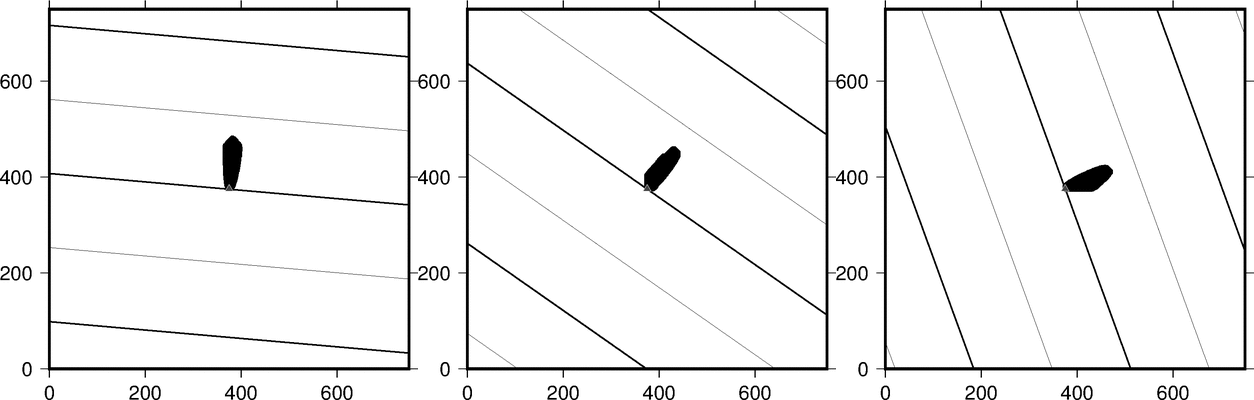
\includegraphics[width=\linewidth]{lava_C_4N_slope}
		\caption{\textit{Rotating slope test for a 4-connected flow algorithm with parent-child relationships which spreads lava proportional to slope (4/P/S). Slope dip is 18$^{\circ}$, dipping 0N, 30N, and 80N from left to right. The flow length and aspect ratio are similar and the flow direction is in the slope direction, so even though the flow is oddly shaped, it passes Level 1 criteria.}}
		\label{fig:slope}
	\end{figure}
	
	Flow runout lengths were calculated by finding the distance between the vent location and the farthest location recorded in the ASCII flow output file. For the eight different transition functions tested, runout length varied between 60-160~m. Flow widths were calculated by finding the farthest point away from a line between the farthest flow point and the vent location on either side. Aspect ratio is calculated as the ratio between runout length and flow width. Direction error is calculated as the degree difference between the slope direction and the direction of the farthest flow point from the vent.
	
	For each flow algorithm, these statistics were calculated 18 times, for each DEM created. Variance for length and aspect ratio were calculated as the ratio of their standard deviations to their means. For instance, if mean runout length for the 18 flows is 100~m and the standard deviation of the 18 lengths is 2~m, the runout length variance is 2\%. The mean direction error is also calculated for the set of flows from each algorithm. These are reported in the table below.

		\begin{center}
			\textbf{DEM Rotation Results}
			\begin{tabular}{l c c c}
				\toprule
				Transition&Run-out&Aspect Ratio&Mean Direction\\
				Function&Variance&Variance&Error\\
				\midrule
				4/P/S &2.7\%&6.7\%&1.2$^{\circ}$\\
				8/P/S &4.4&12.2&0.9\\
				4/N/S &9.6&19.7&1.3\\
				8/N/S &3.9&7.5&0.6\\
				4/P/E &21.6&38.6&14.2\\
				8/P/E &7.2&13.8&5.4\\
				4/N/E &21.6&38.7&14.1\\
				8/N/E &7.2&13.8&5.5\\
				
				\bottomrule
			\end{tabular}
		\end{center}
		
		While with an ideal spreading algorithm, variances and direction error would be 0 under a rotating slope, all spreading algorithms tested performed differently as DEM direction changed. Deciding which pass or fail this test is not necessarily clear from the above results. However, some algorithms can be discarded from their high mean direction error; algorithms with mean direction errors larger than 2$^{\circ}$ can be visually seen, when the flow is mapped, to have a systematic flow direction. This independence from the slope direction suggests that the dummy direction parameter changes the performance of these flows. The flow algorithm with the least flow length variance was the 4-connected, parent-child, slope-proportional strategy implemented in LavaPL.

	\subsection{Level 2: Bingham Flow Approximation}
		
		A flat surface DEM is created with a spatial resolution of 1~m and a height and width of 1300~m to run flows from the centroid. These flows should replicate a circle, which is judged by comparing the number of inundated locations given in the ASCII model output with the number of locations in the DEM within a circle circumscribing the lava flow. A result of 1.0 indicates the flow performs as well as a circle, a result of 0.90 indicates that the flow replicates a circle as well as an octagon, and a result of 0.64 indicates that the flow replicates a circle as well as a square.
		
		\begin{figure}[!h]
		\centering
		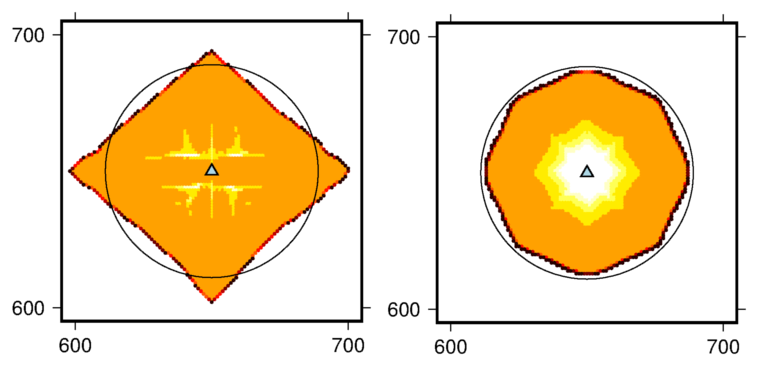
\includegraphics[width=0.7\linewidth]{pancake}
		\caption{\textit{Two flat surface tests for slope proportional spreading algorithms with parent rules. On the left the flow is 4-connected (4/P/S), while on the right the flow is 8-connected (8/P/S).}}
		\label{fig:pancake}
	\end{figure}
	
		
		\begin{center}
			\textbf{Bingham Circle Results}\\
			\begin{tabular}{l c c c}
				\toprule
				Transition Function&Circularity\\
				\midrule
				4/P/S & 0.55\\
				8/P/S & 0.95\\
				4/N/S & 0.55\\
				8/N/S & 0.98\\
				4/P/E & 0.77\\
				4/N/E & 1.00\\
				8/N/E & 0.99\\
				
				\bottomrule
			\end{tabular}
		\end{center}
		
		All but three flow algorithms tested above unambiguously passed the test of performing better than an octagon. Two algorithms unambiguously failed, one of which is the LavaPL algorithm that outperfomed other models in the previous test. In this test 8-connected algorithms outperformed 4-connected algorithms.

	\subsection{Level 3: Replicating Real Flows}
	
	Each transition function was tested over SRTM topography and a TanDEM-X DEM using values gathered from TanDEM-X analysis. Two vents were situated over the topography at UTM coordinates of the two active vents created in the 2012-3 Tolbachik eruption. The total combined volume output from these two vents were 0.38~cubic~km. The residual thickness of the flow is 7.8~m and the pulse volumes were defined as the product of the thickness and the spatial resolution of the underlying DEM. The Jaccard fit for each flow algorithm is listed below for both DEMs.
		\begin{figure}[!h]
			\centering
			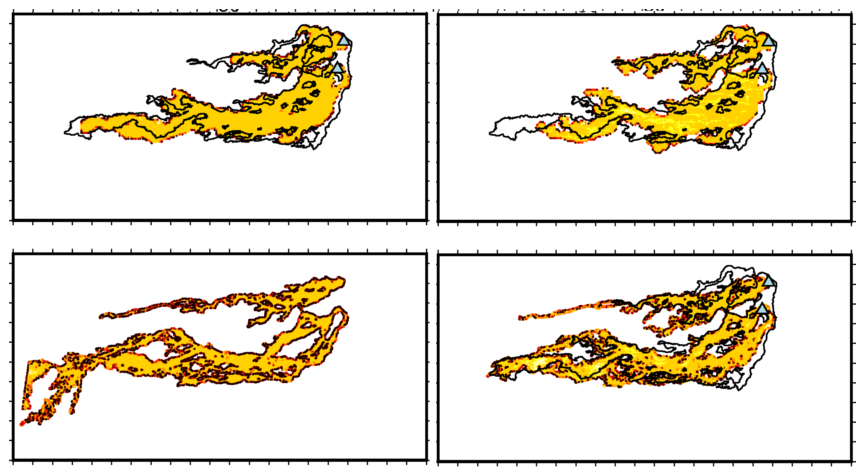
\includegraphics[width=0.7\linewidth]{tolbachik}
			\caption{\textit{Two models run over two DEMs (SRTM, top; TanDEM-X, bottom) in the Tolbachik area. Left: An 8-connected, slope-proportional, no parent algorithm (8/N/S). Right: A 4-connected, equal spreading, no parent algorithm (4/N/E). Most spreading algorithms that had appropriate runout lengths in the SRTM test simulated very long flows over the TanDEM-X DEM. The mapped flow is plotted in black.}}
			\label{fig:tolbachik}
		\end{figure}
		
		\newpage
		\begin{center}
			\textbf{Tolbachik Flow Results}\\
			\begin{tabular}{l c c c}
				\toprule
				Transition Function&SRTM DEM Fit&TanDEM-X DEM Fit\\
				\midrule
				4/P/S & 57.7\%& 53.0\%\\
				8/P/S & 61.1  & 46.8\\
				4/N/S & 57.2  & 44.0\\
				8/N/S & 61.6  & 48.3\\
				4/P/E & 51.2  & 54.2\\
				4/N/E & 54.5  & 55.7\\
				8/N/E & 59.6  & 56.3\\
				
				\bottomrule
			\end{tabular}
		\end{center}

		If success and failure are defined by having a fits of greater or less than 50\%, all models tested would pass for the SRTM DEM and about half would pass for the TanDEM-X DEM. All but one model performed worse on the TanDEM-X DEM.

\section{Discussion and Conclusion}
	A valid model can be determined by elimination. Spreading algorithms that are not slope-proportional spreading methods can be eliminated in the Level 1 test. Of the four remaining algorithms, only 8-connected transition functions succeed in Level 2. Luckily, both of these 8-connected, slope-proportional spreading funtions also perform best in replicating the Tolbachik flows over SRTM. However, they do not pass the 50\% fit test over TanDEM-X.
	
	One reason why most flows do worse over the TanDEM-X DEM could be due to the Pulse Volume used. While this pulse volume is convenient, as it is defined by parameters known \textit{a priori}, it might be essential to test a range of pulse parameters to refine this parameter and find the best possible fit of flows over TanDEM-X data. This is the sixth and final step of the validation guide given by \citet{bayarri2007framework}.
	
	Overall, in all tests 8-connected models outperfom 4-connected models. While equal sharing algorithms outperfom slope-proportional sharing on a flat slope, they fail on a rotating DEM and perform about the same on real topography. There does not seem to be an unambiguously better choice between using parent-child relationships or not. If future tests continue to show similar performance between models with and without parentage, other reasons can be used to choose a model, such as computer run-time. Currently, the perferred model is one that spreads in 8 directions without parentage rules that delivers lava in a slope-proportional fashion.
	
	The strength of the MOLASSES code is that new algorithms, such as those used in the SCIARA model, can be implemented relatively quickly and run through the Benchmarking tests, which are written in Python. Combinations of implementation strategies can also be created on the fly by adjusting the makefile of the MOLASSES code instead of the code itself.
	
\section{Data Statement}
This code is available for free use on GitHub at the USFVolcanology page located at https://github.com/USFvolcanology, while the benchmarking codes can be found at https://github.com/jarichardson/MOLASSES\_benchmarking. The MOLASSES code and the Benchmarking algorithms are kept in seperate self-contained repositories.

%\section{Acknowledgments}
%The development of this code was supported by SSI Grant

\bibliographystyle{plainnat}
\bibliography{lava}

%\begin{figure}
%\centering
%\includegraphics[width=\linewidth]{map_diff}
%\label{fig:map_diff}
%\end{figure}


\end{document}
